\chapter{Learned Quantization\label{cha:chapter3} Schemes}
This chapter introduces two custom learned quantization schemes — approaches that allow models to learn to quantize themselves
with adjustable aggressiveness. The first one, a custom quantization layer featuring a threshold for gradient based scale updates,
will be discussed in the first section. The second scheme, which focuses on custom regularization terms with a configurable penalty rate,
will be covered second.

% ------------------------------------------------------------
% ----------------------- learnedquantization Schemes ----------------------- 
% ------------------------------------------------------------

\section{Nested Quantization Layer}
\label{sec:nestedquantizationlayer}
To separate the quantization logic from the usual structure of NN layers,
we define a nested quantization layer that can be used within a standard one. 
This approach provides usability, making it easy to extend the functionality to other types of layers beyond dense and convolutional ones.
We will first explain the core logic of the nested quantization layer and how it integrates into a model,
followed by a detailed explanation of how the trainable scaling factors are updated.


% -------------------- Implementation details --------------------

\subsection{Core Logic and Structure}
\label{subsec:quantizedconvolutional}

As the name "nested quantization layer" suggests —
this layer is implemented in a way that it is initialized from within a model layer itself.
\\
\\
To explain, let \( P \) be the parameter of a layer (weights, bias or kernel). This \( P \) is used
as the input for the nested quantization layer, where it undergoes quantization based on 
a scaling factor \( s \). In turn, \( s \) is the only trainable parameter of the nested layer itself.
\\
\\
The forward pass of the nested layer performs the following operation:

\[
  P_{reconstructed} = P_{quantized} \cdot s
\]

\noindent where \( P_{quantized} \) is the quantized integer form of \( P \) and is defined as:

\[
  P_{quantized} = floor(\frac{P}{s})
\]

\noindent During backpropagation, the nested layer receives the upstream gradient of
\( P_{reconstructed} \) and passes it downward as is.  This follows the standard STE behaviour
used with non-differentiable discretizers, such as \( floor(\cdot) \) in our case,
as discussed in Subsection \ref{subsec:commonquantizationapproaches}.
\\
\\
For updating the scale factor \( s \) — its own trainable parameter — 
the nested layer utilizes the upstream gradient information of \( P_{\text{reconstructed}} \)
and applies a custom logic, which will be detailed in the next subsection. 
Essentially, this approach solves two problems with one tool — updating both 
\( P \) and \( s \) using the same gradient, although with different logic.
\\
\\
Conceptually, the resulting structure with one or more nested quantization layers is illustrated in Figure \ref{fig:nested_quantization}
on the example of a convolutional layer.
\\
\begin{figure}[h!]
  \centering
  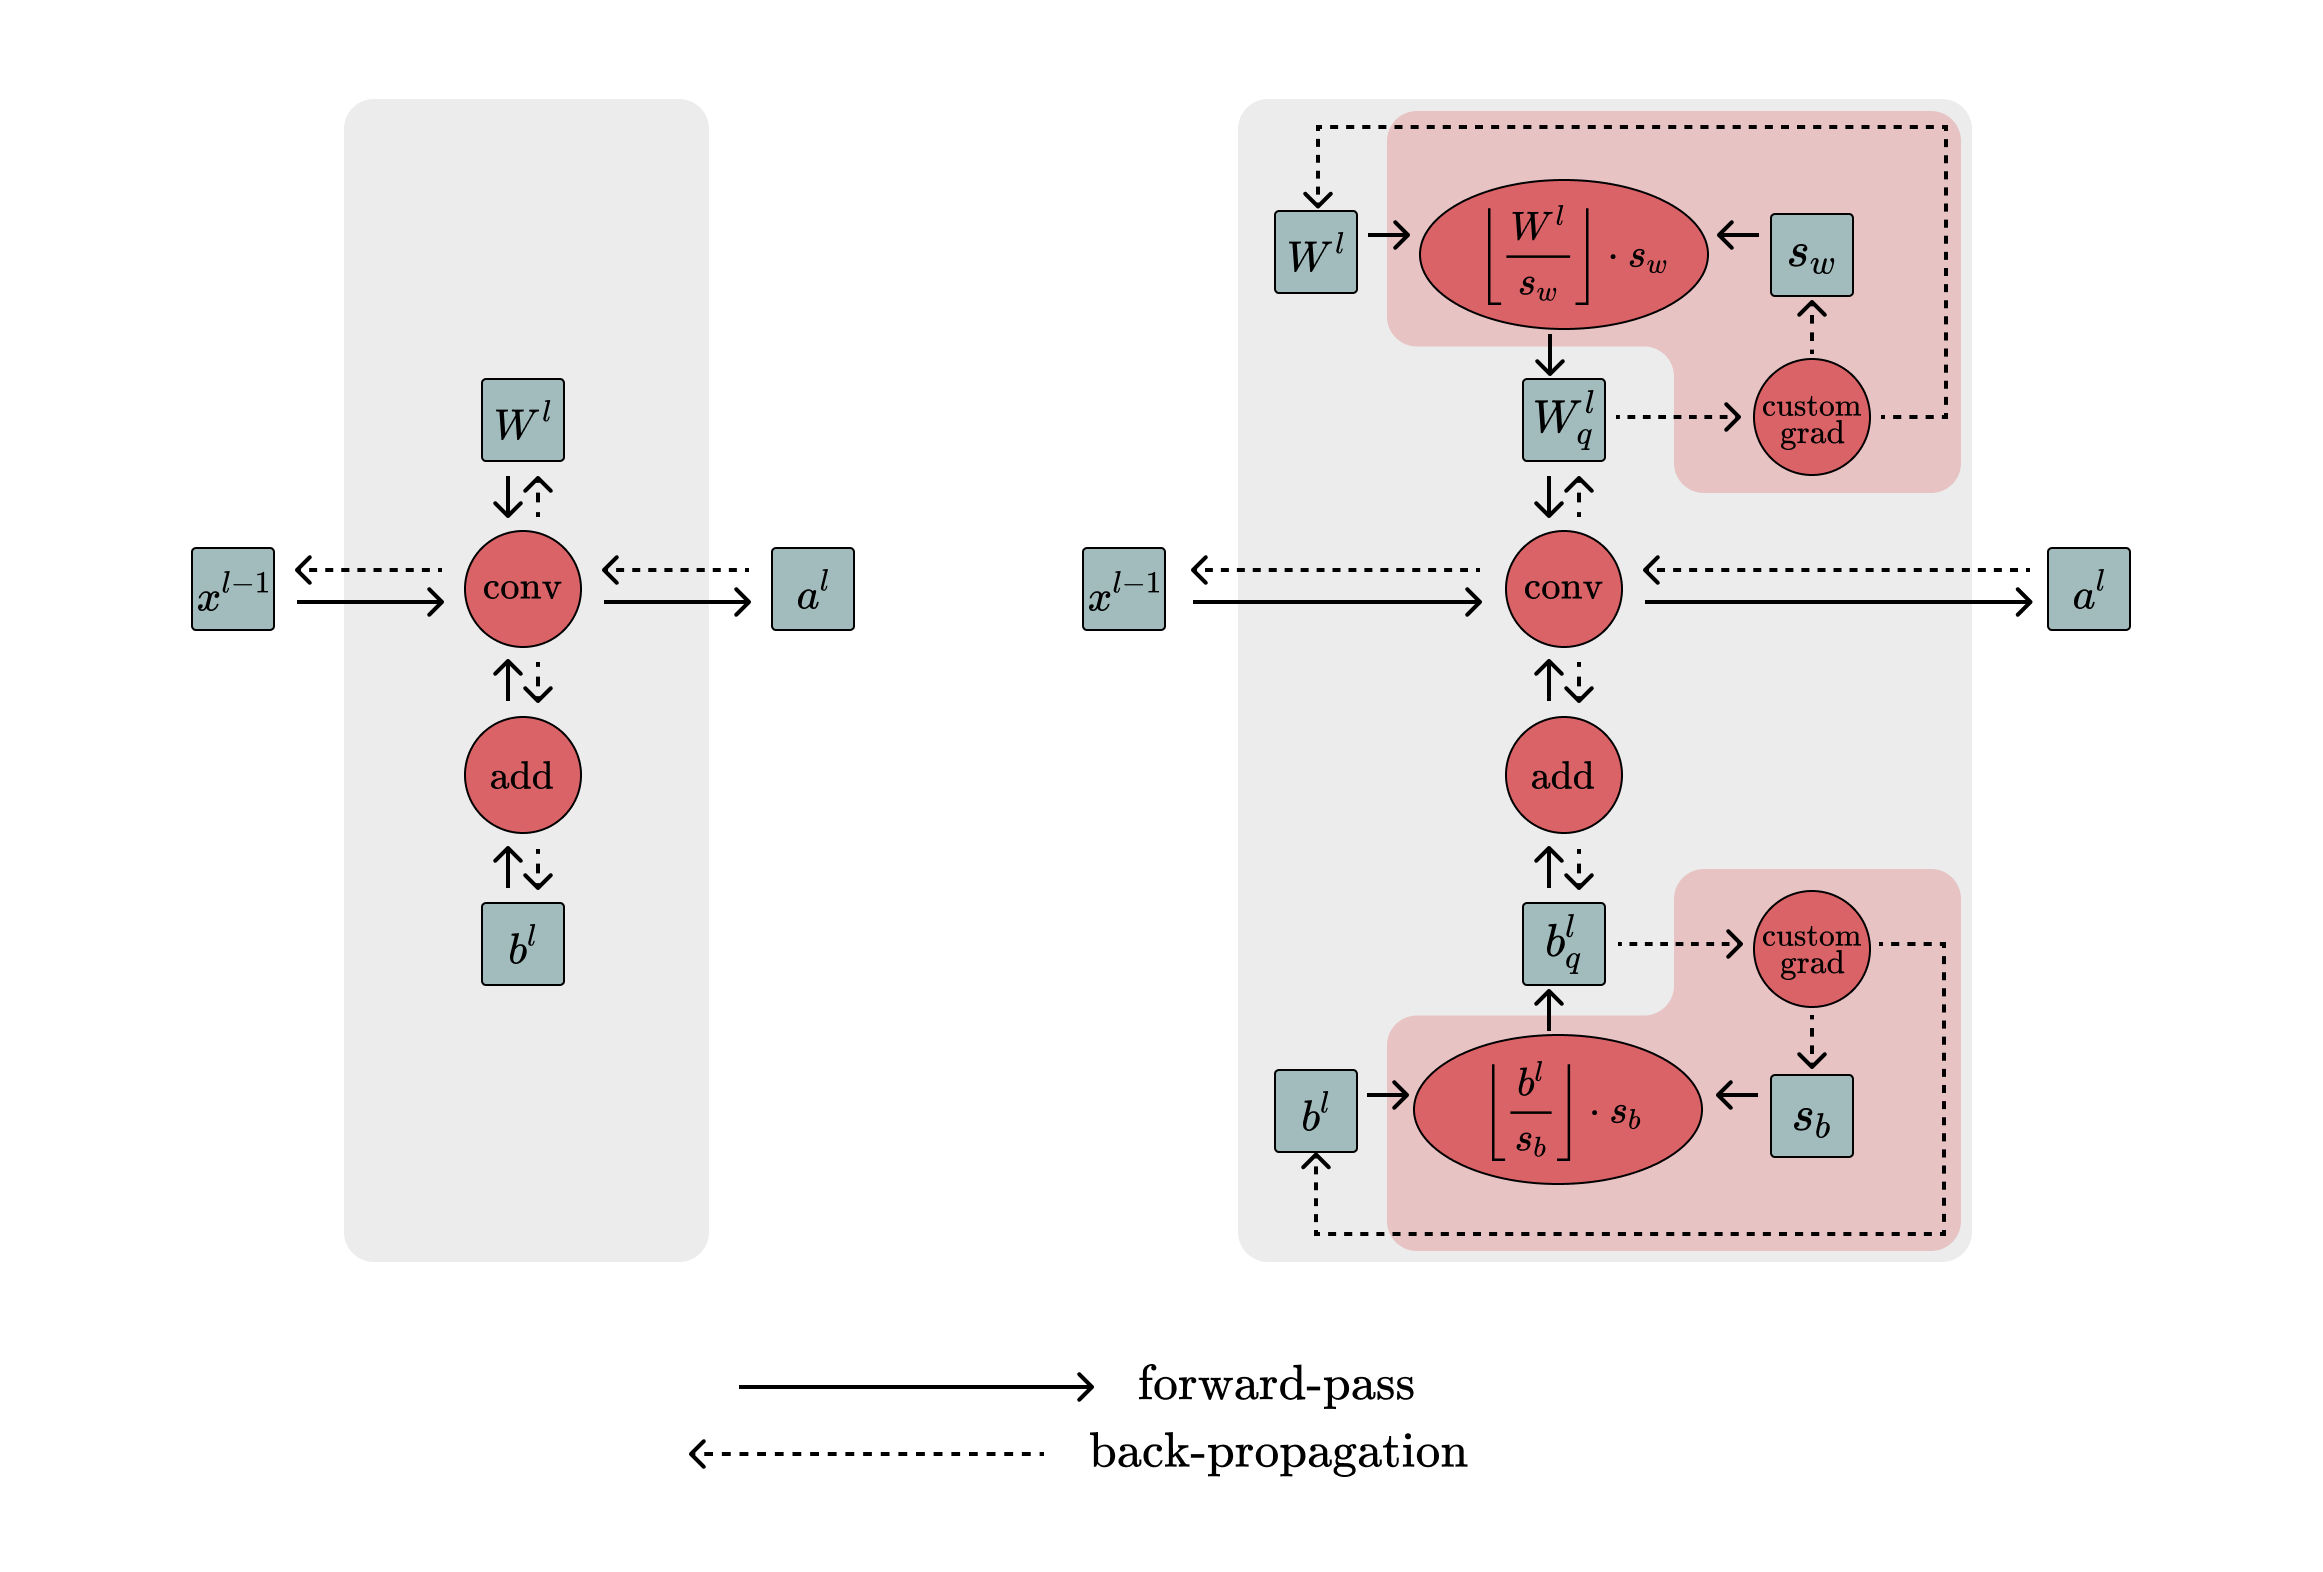
\includegraphics[width=14cm]{nested_quantization_layer.png}
  \caption{A standard convolutional layer (left) and its integration with the nested quantization layer (right) for both weights and bias.
  Quantization logic is applied to weights and biases during the forward pass, with trainable scaling factors 
  updated using custom gradients in the backward pass. Parameter gradients are passed downward as is.}
  \label{fig:nested_quantization}
\end{figure}

\noindent Since the scaling factor \( s \) can have different shapes and be applied at varying levels of granularity,
we have enabled scalar, row-wise, and column-wise application granularity for dense layers,
as shown in Figure \ref{fig:scaler-application-dense}. 
For convolutional layers, we additionally support channel-wise granularity,
corresponding to the first four scenarios in Figure \ref{fig:granularity-conv2d}.
\\
\begin{figure}[h!]
  \centering
  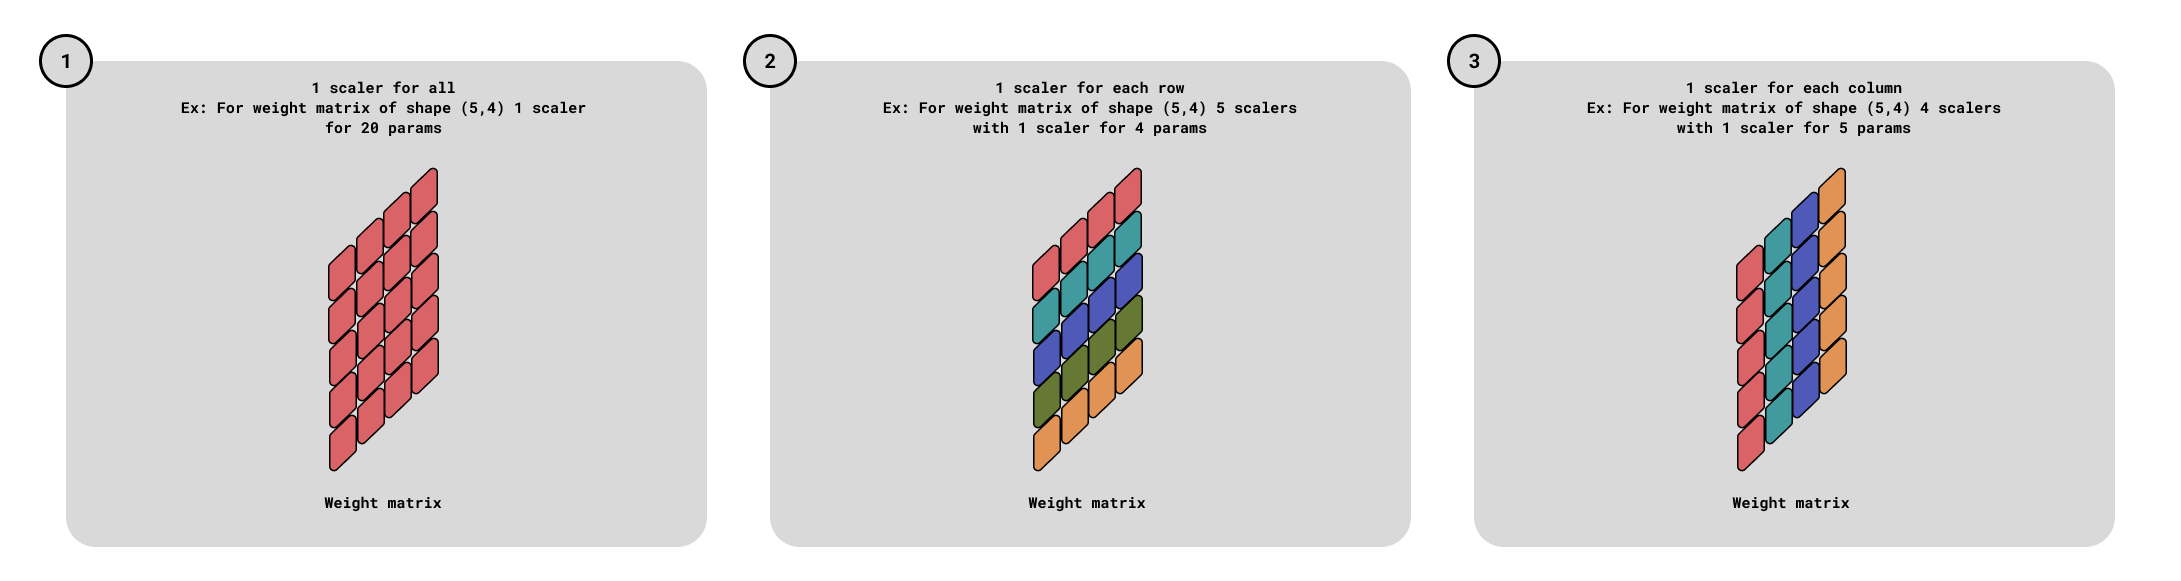
\includegraphics[width=14cm]{Scaler-application-dense.png}
  \caption{A demonstration of the varying applications of scaling factors, ranging from a single scalar applied to the entire weight matrix (1) to row-wise and column-wise application of vector scalers.}
  \label{fig:scaler-application-dense}
\end{figure}

\noindent The nested layer is built upon Tensorflow's \texttt{tf.keras.Layer} class,
which serves as the base for all Keras layers. The gradient calculation logic is wrapped
in Tensorflow's \texttt{tf.custom\_gradient} decorator, allowing proper functioning of the 
model's computational graph. Dense and convolutional layers have been implemented as 
\texttt{tf.keras.Layer} objects with minimal adjustments as well to incorporate the nested layers logic.

% -------------------- concept and design --------------------

\subsection{Learned Scale Factor}
\label{subsec:learnedscalefactor}

For the trainable scale factor \( s \), we define a custom gradient formula. 
The gradient of the loss with respect to \( s \), denoted as \( \nabla_s L \), is computed as:
\[
\nabla_s L = g_s \cdot m,
\]
Let's consider both multiplication terms separately. \(  g_s  \) is the main "decision maker" on whether to
increase the scale and, therefore, quantize more. It is based on a hyperparameter threshold  \(  \lambda  \),
which is compared against the ratio \(  r  \).

\[
g_s = 
\begin{cases} 
0, & \text{if } r \geq \lambda, \\
- \tanh(\lambda - r), & \text{if } r < \lambda,
\end{cases}
\]

\noindent In turn, \(  r  \) is the ratio between the upstream gradient of the layer's reconstructed parameter with respect to the loss
and its absolute value (for simplicity, we done \( P_{reconstructed}\) as \(P_r\)):

\[
r = \frac{\left| \nabla_{P_{r}} L \right|}{\max(\epsilon, \left| P_r \right|)}
\]

\noindent In essence, it conveys the relative impact of the gradient on the parameter's value.
A large ratio indicates that the parameter is not ready for aggressive quantization
because small perturbations can lead to significant changes in its optimization.
Conversely, parameters with a small \(  r  \) are better candidates
for quantization since they are less sensitive.
\\
\\
The decision to replace \( P_r \) with \( \epsilon \) when \( P_r = 0 \)
ensures that the corresponding \( r \) becomes large,
effectively resisting quantization. This behavior is valid regardless of the parameter's sensitivity
 — if the zero parameter is sensitive, quantization could disrupt future optimization steps,
 and if it is not sensitive, quantization adds no value since \( s \) has a positive non-zero constraint 
 and \( \frac{P}{s} \) will remain zero.
\\
\\
The motivation behind using \( tanh(\cdot) \) primarily stems from two key reasons. 
First, it is bounded (in our use case, to \( [-1, 0) \)), which prevents excessive gradient magnitudes.
Second, unlike sigmoid, it does not require any additional rescaling since it is
symmetric around \( 0 \). An additional point is that \( tanh(\cdot) \) saturates comparably faster,
potentially allowing for more decisive gradients,
but it is uncertain how much influence this has.
\\
\\
Now that \( g_s \) is covered, let's take a look at \( m \) defined as:

\[
m = \max\left(\left| P_{\text{quantized}} \right|\right) 
\]

\noindent where the shape of \( m \) corresponds to the shape of \( s \).
For example, if \( s \) is a row-wise scaler, then \( m  \) will hold
the maximum value from each row of \( \left| P_{quantized} \right|\).
Similarly if  \( s \) is a scalar scaler, then \( m \) represents
the maximum across the entire layer parameter.
\\
\\
A larger \( m \) indicates a wider range of quantized values,
implying the parameter can tolerate coarser quantization.
In contrast, a smaller \( m \) means a narrower range,
where aggressive quantization could be rather harmful.
As a result, by multiplying \( g_s\) with \( m \), 
the adjustment to the scale becomes proportional to the parameter's range.
This encourages more aggressive quantization for parameters with larger ranges
while being more conservative for smaller ones.
\\
\\
To sum this part up, the intuition is that the gradient adjustment for the scale factor
\( s \) adapts dynamically based on both the sensitivity of the parameter ( \( g_s\) )
and its range ( \( m \) ). Sensitive parameters are left with a "zero vote,"
while the less sensitive ones have a say on how much quantization they can tolerate.
\\
\\
The final touch is that the scale gradients are initially calculated for each parameter value
but are then aggregated along the corresponding granularity axes.
This reflects the collective behavior of parameters within the same granularity,
where only those deemed quantizable and with a meaningful "say" contribute to the overall adjustment,
while sensitive parameters express their resistance with a "zero vote."
\\
\\
In Chapter \ref{cha:chapter4}, we will present experimental results for different values of 
\( \lambda \), offering guidance on the optimal values for both dense and convolutional layers.


\section{Custom Loss Functions}
\label{sec:customloss}

\subsection{Penalty for Inverse Scale Factor Magnitude} 
\label{subsec:scaleinverse}

\subsection{Constraint on Bin Count for Quantization}
\label{subsec:maxbin}

\subsection{Deviation between Quantized and Original Values}
\label{subsec:difference}